\documentclass[12pt,letterpaper]{article}
\usepackage[margin=3cm]{geometry}
\usepackage{graphicx}
\usepackage{enumitem}
\usepackage{array}
\usepackage{longtable}
\usepackage{tikz}
\usepackage[colorlinks=true,linkcolor=black,urlcolor=blue,citecolor=black]{hyperref}
\usepackage{xurl}
\usepackage{titlesec}
\usepackage{parskip}
\usepackage{xcolor}
\titleformat{\section}{\large\bfseries}{\thesection.}{0.5em}{}
\titleformat{\subsection}{\normalsize\bfseries}{\thesubsection.}{0.5em}{}
\emergencystretch=2em
\setlist{itemsep=2pt,topsep=3pt}

\begin{document}

\begin{titlepage}
\centering

\includegraphics[width=4cm]{escudo.png}\\[0.6cm]
{\Large\bfseries Universidad de Sonora}\\[0.3cm]
{\large Licenciatura en Ciencias de la Computación}\\[1.5cm]
{\LARGE\bfseries Tarea IPv6}\\[0.4cm]
{\large Protocolo de Internet versión 6}\\[1.5cm]
\begin{tabular}{rl}
\textbf{Materia:} & Redes de Computadoras I\\
\textbf{Periodo:} & 2026-2\\
\textbf{Profesor:} & Dr. Donald José Rodríguez Úbeda\\
\end{tabular}\\[1.5cm]
{\large\bfseries Integrantes del equipo}\\[0.3cm]
\begin{tabular}{ll}
Angel Alberto Amaya Soria & Expediente 223210350\\
Angel Fernando Bórquez Guerrero & Expediente 219208106\\
Emily Margarita Beltrán Zazueta & Expediente 223203546\\
Gabriela Aydee Miranda & Expediente 222220740\\
Javier Leonardo Miranda Sánchez & Expediente 223215039\\
\end{tabular}\\[1.5cm]
Hermosillo, Sonora \hfill Noviembre de 2026
\end{titlepage}

\tableofcontents
\newpage

\section{¿Qué es IPv6?}
IPv6 (\emph{Internet Protocol, version 6}) es la versión del Protocolo de Internet que sustituye a IPv4. Se diseñó sobre todo para resolver el agotamiento de las direcciones IPv4, que tienen 32 bits (unos $4.3\times10^{9}$ direcciones), usando direcciones de 128 bits, es decir, unos $3.4\times10^{38}$ (Deering \& Hinden, 2017; Tanenbaum \& Wetherall, 2011). Además de ampliar el espacio de direcciones, simplifica el encabezado del paquete y mejora el soporte para multidifusión, autoconfiguración y extensiones.

Su adopción ha sido gradual: en abril de 2026 las mediciones de Google mostraban que cerca del 50\,\% de sus usuarios accedían a sus servicios por IPv6, mientras que la medición de APNIC daba 42\,\% de capacidad mundial (Michaelson, 2026). Hoy convive con IPv4 en lo que se ha llamado una Internet de dos protocolos.

\section{¿Sus direcciones son compatibles con IPv4?}
\textbf{No directamente.} IPv6 es un protocolo distinto: usa otro formato de encabezado y direcciones de otro tamaño, por lo que un nodo que solo habla IPv4 no puede comunicarse con uno que solo habla IPv6 sin un mecanismo intermedio (Kurose \& Ross, 2017).

\textbf{Formato de las direcciones.} Se escriben como ocho grupos de hasta cuatro dígitos hexadecimales separados por dos puntos, y una sola secuencia de grupos en cero puede abreviarse con \texttt{::}. Por ejemplo, \texttt{2001:0db8:0000:0000:0000:0000:0000:0001} se abrevia como \texttt{2001:db8::1}. Existen tres tipos: \emph{unicast} (una interfaz), \emph{anycast} (la interfaz más cercana de un grupo) y \emph{multicast} (todas las interfaces de un grupo); no hay direcciones de difusión (\emph{broadcast}), cuyo papel pasa a la multidifusión. También hay direcciones especiales, como el \emph{loopback} \texttt{::1} y las locales de enlace \texttt{fe80::/10} (Hinden \& Deering, 2006).

\textbf{Mecanismos de convivencia.} El protocolo incluye una forma de representar direcciones IPv4 dentro de IPv6 (las direcciones \emph{IPv4-mapped}, de la forma \texttt{::ffff:a.b.c.d}), pero la compatibilidad real se logra con técnicas de transición:
\begin{itemize}
\item \textbf{Doble pila} (\emph{dual stack}): los equipos ejecutan IPv4 e IPv6 al mismo tiempo (Nordmark \& Gilligan, 2005).
\item \textbf{Túneles}: los paquetes IPv6 viajan encapsulados dentro de paquetes IPv4 para cruzar redes que aún no soportan IPv6 (Nordmark \& Gilligan, 2005).
\item \textbf{Traducción} (NAT64 y DNS64): un traductor permite que clientes solo IPv6 accedan a servidores IPv4 (Bagnulo et al., 2011a, 2011b).
\end{itemize}

\section{¿Cómo se resuelve el problema de redireccionamiento?}
En IPv6 el reenvío de paquetes (enrutamiento) se hace más eficiente y la tabla de rutas más pequeña por varias decisiones de diseño:
\begin{itemize}
\item \textbf{Direccionamiento jerárquico y agregable.} Las direcciones globales tienen un prefijo de enrutamiento global, un identificador de subred y un identificador de interfaz de 64 bits. Los proveedores reciben bloques grandes y los resumen en una sola ruta, lo que reduce el tamaño de las tablas de los enrutadores (Hinden \& Deering, 2006).
\item \textbf{Encabezado simple de longitud fija.} Tiene 40 bytes y no incluye suma de verificación, por lo que cada enrutador hace menos trabajo por paquete (Deering \& Hinden, 2017).
\item \textbf{Sin fragmentación en los enrutadores.} Solo el origen fragmenta; los enlaces deben soportar una MTU mínima de 1280 bytes y el origen descubre la MTU de la ruta (Deering \& Hinden, 2017; McCann et al., 2017).
\item \textbf{Descubrimiento de vecinos (\emph{Neighbor Discovery}).} Reemplaza a ARP y también incluye el mensaje \emph{Redirect}, con el que un enrutador informa a un equipo de que existe un mejor primer salto hacia un destino (Narten et al., 2007a).
\item \textbf{Protocolos de enrutamiento adaptados.} OSPFv3 y las extensiones multiprotocolo de BGP reparten rutas IPv6 (Coltun et al., 2008; Bates et al., 2007). La cabecera de enrutamiento permite además especificar nodos intermedios por los que debe pasar el paquete (Deering \& Hinden, 2017).
\end{itemize}

\section{¿Cómo está conformado un paquete en IPv6?}
Un paquete IPv6 se compone de un encabezado base de 40 bytes (320 bits), cero o más encabezados de extensión y la carga útil (Deering \& Hinden, 2017).

\begin{center}
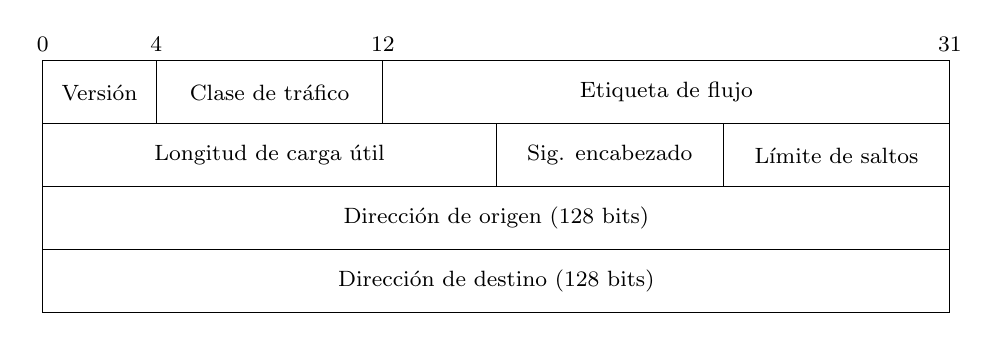
\begin{tikzpicture}[x=0.36cm,y=0.8cm,font=\footnotesize]
\draw (0,0) rectangle (4,-1) node[midway]{Versión};
\draw (4,0) rectangle (12,-1) node[midway]{Clase de tráfico};
\draw (12,0) rectangle (32,-1) node[midway]{Etiqueta de flujo};
\draw (0,-1) rectangle (16,-2) node[midway]{Longitud de carga útil};
\draw (16,-1) rectangle (24,-2) node[midway]{Sig. encabezado};
\draw (24,-1) rectangle (32,-2) node[midway]{Límite de saltos};
\draw (0,-2) rectangle (32,-3) node[midway]{Dirección de origen (128 bits)};
\draw (0,-3) rectangle (32,-4) node[midway]{Dirección de destino (128 bits)};
\node[above] at (0,0) {0};
\node[above] at (32,0) {31};
\node[above] at (4,0) {4};
\node[above] at (12,0) {12};
\end{tikzpicture}\\[3pt]
{\footnotesize Figura 1. Encabezado base de IPv6 (ancho de 32 bits; las direcciones ocupan cuatro palabras de 32 bits cada una).}
\end{center}


\newpage
{\small
\renewcommand{\arraystretch}{1.12}
\begin{longtable}[c]{|>{\raggedright\arraybackslash}p{3.4cm}|c|>{\raggedright\arraybackslash}p{8.2cm}|}
\hline
\textbf{Campo} & \textbf{Bits} & \textbf{Propósito}\\
\hline
Versión & 4 & Identifica la versión del protocolo; vale 6.\\ \hline
Clase de tráfico (\emph{Traffic Class}) & 8 & Permite distinguir clases o prioridades de paquetes para darles un trato diferenciado.\\ \hline
Etiqueta de flujo (\emph{Flow Label}) & 20 & Marca los paquetes que pertenecen a un mismo flujo para que los enrutadores los traten igual, por ejemplo, el mismo camino.\\ \hline
Longitud de carga útil (\emph{Payload Length}) & 16 & Tamaño en bytes de lo que sigue al encabezado base, incluidos los encabezados de extensión.\\ \hline
Siguiente encabezado (\emph{Next Header}) & 8 & Indica qué sigue: un encabezado de extensión o el protocolo de capa superior (por ejemplo, TCP o UDP).\\ \hline
Límite de saltos (\emph{Hop Limit}) & 8 & Cada nodo que reenvía el paquete lo disminuye en uno; al llegar a cero se descarta. Evita que un paquete circule indefinidamente (equivale al TTL de IPv4).\\ \hline
Dirección de origen & 128 & Dirección de quien envía el paquete.\\ \hline
Dirección de destino & 128 & Dirección de quien debe recibirlo (puede no ser el destino final si hay cabecera de enrutamiento).\\ \hline
\end{longtable}
\vspace{-8pt}\begin{center}{\footnotesize Tabla 1. Campos del encabezado base de IPv6 (Deering \& Hinden, 2017).}\end{center}}

\textbf{Encabezados de extensión.} Las opciones que en IPv4 iban en el encabezado se mueven a encabezados opcionales que se encadenan mediante el campo Siguiente encabezado. Los principales son: opciones salto por salto (valor 0), enrutamiento (43), fragmentación (44), opciones de destino (60), autenticación (AH) y carga de seguridad encapsulada (ESP). Se recomienda ponerlos en ese orden, y los enrutadores intermedios solo procesan los que les corresponden (Deering \& Hinden, 2017).

\textbf{Diferencias con IPv4.} Desaparecen los campos de longitud del encabezado, identificación, banderas, desplazamiento de fragmento, suma de verificación y opciones. El tipo de servicio pasó a ser Clase de tráfico, el TTL a Límite de saltos, y el campo Protocolo a Siguiente encabezado (Tanenbaum \& Wetherall, 2011).

\section{Ventajas y desventajas}
\subsection{Ventajas}
\begin{itemize}
\item \textbf{Espacio de direcciones prácticamente inagotable}, que permite que cada dispositivo tenga una dirección global y reduce la necesidad de NAT.
\item \textbf{Encabezado más simple y de tamaño fijo}, con menos procesamiento en los enrutadores.
\item \textbf{Mejor enrutamiento}: direcciones agregables y tablas de rutas más pequeñas.
\item \textbf{Autoconfiguración}: los equipos pueden obtener su dirección sin servidor (SLAAC) (Thomson et al., 2007).
\item \textbf{Multidifusión y \emph{anycast} integrados}, en lugar de difusión.
\item \textbf{Extensible} gracias a los encabezados de extensión, y con soporte para IPsec.
\end{itemize}
\subsection{Desventajas}
\begin{itemize}
\item \textbf{No es compatible con IPv4}: la transición exige doble pila, túneles o traducción, lo que agrega complejidad y costo (Nordmark \& Gilligan, 2005).
\item \textbf{Mayor sobrecarga por paquete}: el encabezado mínimo mide 40 bytes contra 20 de IPv4.
\item \textbf{Direcciones largas}, más difíciles de recordar, escribir y administrar a mano.
\item \textbf{Privacidad}: si la dirección se deriva de la dirección MAC, se puede rastrear al dispositivo; para evitarlo existen direcciones temporales (Narten et al., 2007b).
\item \textbf{Costo de migración}: hay que actualizar equipos, software, cortafuegos y personal, y mientras tanto la red debe mantener dos protocolos.
\end{itemize}

\section{Conclusión}
IPv6 resuelve de raíz el agotamiento de direcciones de IPv4 y, al mismo tiempo, simplifica el reenvío de paquetes con un encabezado fijo y direcciones agregables. Su principal obstáculo no es técnico sino de transición: al no ser compatible con IPv4, ambos protocolos deben convivir durante años, y por eso su adopción es gradual aunque ya alcanza aproximadamente la mitad de los usuarios (Michaelson, 2026).

\newpage
\section*{Referencias}
\addcontentsline{toc}{section}{Referencias}
\begin{itemize}[leftmargin=1.5em,itemsep=3pt]
\item[] Bagnulo, M., Matthews, P., \& van Beijnum, I. (2011a). \emph{RFC 6146: Stateful NAT64: Network address and protocol translation from IPv6 clients to IPv4 servers}. Internet Engineering Task Force.
\item[] Bagnulo, M., Sullivan, A., Matthews, P., \& van Beijnum, I. (2011b). \emph{RFC 6147: DNS64: DNS extensions for network address translation from IPv6 clients to IPv4 servers}. Internet Engineering Task Force.
\item[] Bates, T., Chandra, R., Katz, D., \& Rekhter, Y. (2007). \emph{RFC 4760: Multiprotocol extensions for BGP-4}. Internet Engineering Task Force.
\item[] Coltun, R., Ferguson, D., Moy, J., \& Lindem, A. (2008). \emph{RFC 5340: OSPF for IPv6}. Internet Engineering Task Force.
\item[] Deering, S., \& Hinden, R. (2017). \emph{RFC 8200: Internet Protocol, version 6 (IPv6) specification}. Internet Engineering Task Force. \url{https://datatracker.ietf.org/doc/html/rfc8200}
\item[] Hinden, R., \& Deering, S. (2006). \emph{RFC 4291: IP version 6 addressing architecture}. Internet Engineering Task Force.
\item[] Kurose, J. F., \& Ross, K. W. (2017). \emph{Computer networking: A top-down approach} (7.ª ed.). Pearson.
\item[] McCann, J., Deering, S., Mogul, J., \& Hinden, R. (2017). \emph{RFC 8201: Path MTU discovery for IP version 6}. Internet Engineering Task Force.
\item[] Michaelson, G. (2026, 28 de abril). Google hits 50\% IPv6. \emph{APNIC Blog}. \url{https://blog.apnic.net/2026/04/28/google-hits-50-ipv6}
\item[] Narten, T., Draves, R., \& Krishnan, S. (2007b). \emph{RFC 4941: Privacy extensions for stateless address autoconfiguration in IPv6}. Internet Engineering Task Force.
\item[] Narten, T., Nordmark, E., Simpson, W., \& Soliman, H. (2007a). \emph{RFC 4861: Neighbor discovery for IP version 6 (IPv6)}. Internet Engineering Task Force.
\item[] Nordmark, E., \& Gilligan, R. (2005). \emph{RFC 4213: Basic transition mechanisms for IPv6 hosts and routers}. Internet Engineering Task Force.
\item[] Tanenbaum, A. S., \& Wetherall, D. J. (2011). \emph{Computer networks} (5.ª ed.). Prentice Hall.
\item[] Thomson, S., Narten, T., \& Jinmei, T. (2007). \emph{RFC 4862: IPv6 stateless address autoconfiguration}. Internet Engineering Task Force.
\end{itemize}
\end{document}
